\documentclass[a4paper]{article}
\usepackage[a4paper,left=2cm,right=2cm,top=0.5cm,bottom=0.5cm,includehead,includefoot,headheight=0.1cm,heightrounded]{geometry}
\usepackage{amsmath}
\usepackage{amssymb}
\usepackage{graphics}
\usepackage{graphicx}
\usepackage[table,xcdraw]{xcolor}
\usepackage{float}
\usepackage{fontawesome}
\usepackage{ragged2e}
\usepackage{titlesec}
\usepackage{tikz}
\usepackage{pdfpages}
\usepackage[title]{appendix}
\usepackage[export]{adjustbox}
\usetikzlibrary{automata, positioning, shapes.symbols, arrows, chains, calc}
\usepackage[nottoc,numbib]{tocbibind}
\usepackage{shellesc}
\usepackage{minted}
\usepackage{listings}
\usepackage[hidelinks]{hyperref}
\usepackage[osfigures]{opensans}
\usepackage{lastpage}
\usepackage{fancyhdr}
\usepackage{mdframed}
\usepackage{bm}
\usepackage{array}
\usepackage{enumitem}
\usepackage[round]{natbib}
\usepackage{environ}
\usepackage{varwidth}
\usepackage{mathtools}
\usepackage{pagecolor}
\usepackage{wrapfig}
\usepackage{csquotes}
\usepackage[super]{nth}
\newlength{\MyMdframedWidthTweak}%
\NewEnviron{MyMdframed}[1][]{%
    \setlength{\MyMdframedWidthTweak}{\dimexpr%
        +\mdflength{innerleftmargin}
        +\mdflength{innerrightmargin}
        +\mdflength{leftmargin}
        +\mdflength{rightmargin}
    }%
    \savebox0{%
        \begin{varwidth}{\dimexpr\linewidth-\MyMdframedWidthTweak\relax}%
            \BODY
        \end{varwidth}%
    }%
    \begin{mdframed}[
        backgroundcolor=lightgrey,
        topline=true,
        rightline=false,
        leftline=false,
        linecolor=id7-aubergine,
        userdefinedwidth=\dimexpr\wd0+\MyMdframedWidthTweak\relax, 
        #1]
        \usebox0
    \end{mdframed}
}
\DeclarePairedDelimiter\abs{\lvert}{\rvert}%
\title{}
\author{}
\definecolor{infogreen}{rgb}{0.153, 0.682, 0.376}
\definecolor{id7-aubergine}{HTML}{5B3069}
\definecolor{id7-gray}{HTML}{3F4246}
\definecolor{body-text}{HTML}{333333}
\definecolor{id7-gold}{HTML}{886C11}
\definecolor{id7-burnt-orange}{HTML}{A14418}
\definecolor{id7-ruby-red}{HTML}{89102C}
\definecolor{id7-emerald-green}{HTML}{797906}
\definecolor{id7-sky-blue}{HTML}{204F79}
\definecolor{id7-sky-blue-accent}{HTML}{4d7294}
\definecolor{id7-sky-blue-tint}{HTML}{bccad7}
\definecolor{skyblue}{rgb}{0.125, 0.31, 0.475}
\setlength{\parindent}{0em}
\setlength{\parskip}{1em}
\definecolor{todocolor}{rgb}{0.688,0.8176,0.93137}
\newcommand{\todobox}[1] {\colorbox{todocolor}{\parbox{\textwidth}{\vspace{.75\baselineskip}\centering\parbox{0.95\textwidth}{\faicon{lightbulb-o} \textbf{TODO:} #1\vspace{.75\baselineskip}}}}}
\newcommand{\readbox}[1] {\colorbox{infogreen}{\parbox{\textwidth}{\vspace{.75\baselineskip}\centering\parbox{0.95\textwidth}{\textcolor{white}{\faicon{book} \textbf{#1}\vspace{.75\baselineskip}}}}}}
\def\labelitemi{\textcolor{id7-aubergine}{\textbullet}}
\def\labelitemii{\textcolor{id7-aubergine}{$\circ$}}
\def\labelitemiii{\textcolor{id7-aubergine}{--}}
\definecolor{infogreenlight}{rgb}{0.75,1,0.75}
\definecolor{termbg}{HTML}{232729}

\newcommand{\infobox}[1] {\colorbox{id7-sky-blue-tint}{\parbox{\textwidth}{\vspace{.75\baselineskip}\centering\parbox{0.95\textwidth}{\faicon{info-circle} \sffamily#1\vspace{.75\baselineskip}}}}}

\newcommand{\termbox}[1] {\colorbox{termbg}{\parbox{\textwidth}{\vspace{.75\baselineskip}\centering\parbox{0.95\textwidth}{ \sffamily#1\vspace{.75\baselineskip}}}}}

\newcommand{\boxedfigure}[2]{\begin{MyMdframed}\begin{figure}[H]
            \begin{center}\vspace{2em}\includegraphics[width=0.5\textwidth]{#1}\end{center}
            \caption{#2}
\end{figure}\end{MyMdframed}}

\newcommand{\widthboxedfigure}[3]{\begin{MyMdframed}\begin{figure}[H]
            \begin{center}\vspace{2em}\includegraphics[width=#3\textwidth]{#1}\end{center}
            \caption{#2}
\end{figure}\end{MyMdframed}}

\newcommand{\infoinlineicon}[1] {\colorbox{infogreenlight}{\faicon{info-circle} #1}}

\newcommand{\infoinline}[1] {\colorbox{infogreenlight}{#1}}

\definecolor{orange}{rgb}{0.9529,0.85176,0.5070588}

\newcommand{\warnbox}[1] {\colorbox{orange}{\parbox{\textwidth}{\vspace{.75\baselineskip}\centering\parbox{0.95\textwidth}{\faicon{exclamation-triangle} #1\vspace{.75\baselineskip}}}}}

\newcommand{\warninlineicon}[1] {\colorbox{orange}{\faicon{exclamation-triangle} #1}}

\newcommand{\warninline}[1] {\colorbox{orange}{#1}}

\titleformat{\section}
{\normalfont\sffamily\huge\color{id7-aubergine}}
{\thesection. }{0em}{}

\titleformat{\subsection}
{\normalfont\Large\sffamily\color{id7-aubergine}}
{\thesection}{0em}{}

\titleformat{\subsubsection}
{\normalfont\large\sffamily\color{id7-aubergine}}
{\thesection}{0em}{}
\fancyhf{}
\pagestyle{fancy}
\renewcommand{\headrulewidth}{0pt}
\lfoot{\textcolor{grey}{Adam Williams}}
\rfoot{\textcolor{grey}{Page \thepage{} of \pageref{LastPage}}}

\renewcommand*\footnoterule{\noindent\makebox[\textwidth]{
\includegraphics[width=\paperwidth]{divider}}}

\definecolor{grey}{rgb}{0.5,0.5,0.5}
\definecolor{lightgrey}{rgb}{0.96,0.96,0.96}

\def \spacedrule {\textcolor{id7-aubergine}{\hrule}\vspace{1em}}
\def \thedate {November \nth{15} 2018}
\lhead{\textcolor{grey}{\thedate}}
\rhead{\textcolor{grey}{Progress Report}}
% ======================

\begin{document}
    
\newgeometry{margin=0in}
\begin{titlepage}
    
    \tikz[remember picture,overlay] \node[opacity=1,inner sep=0pt] at (current page.center){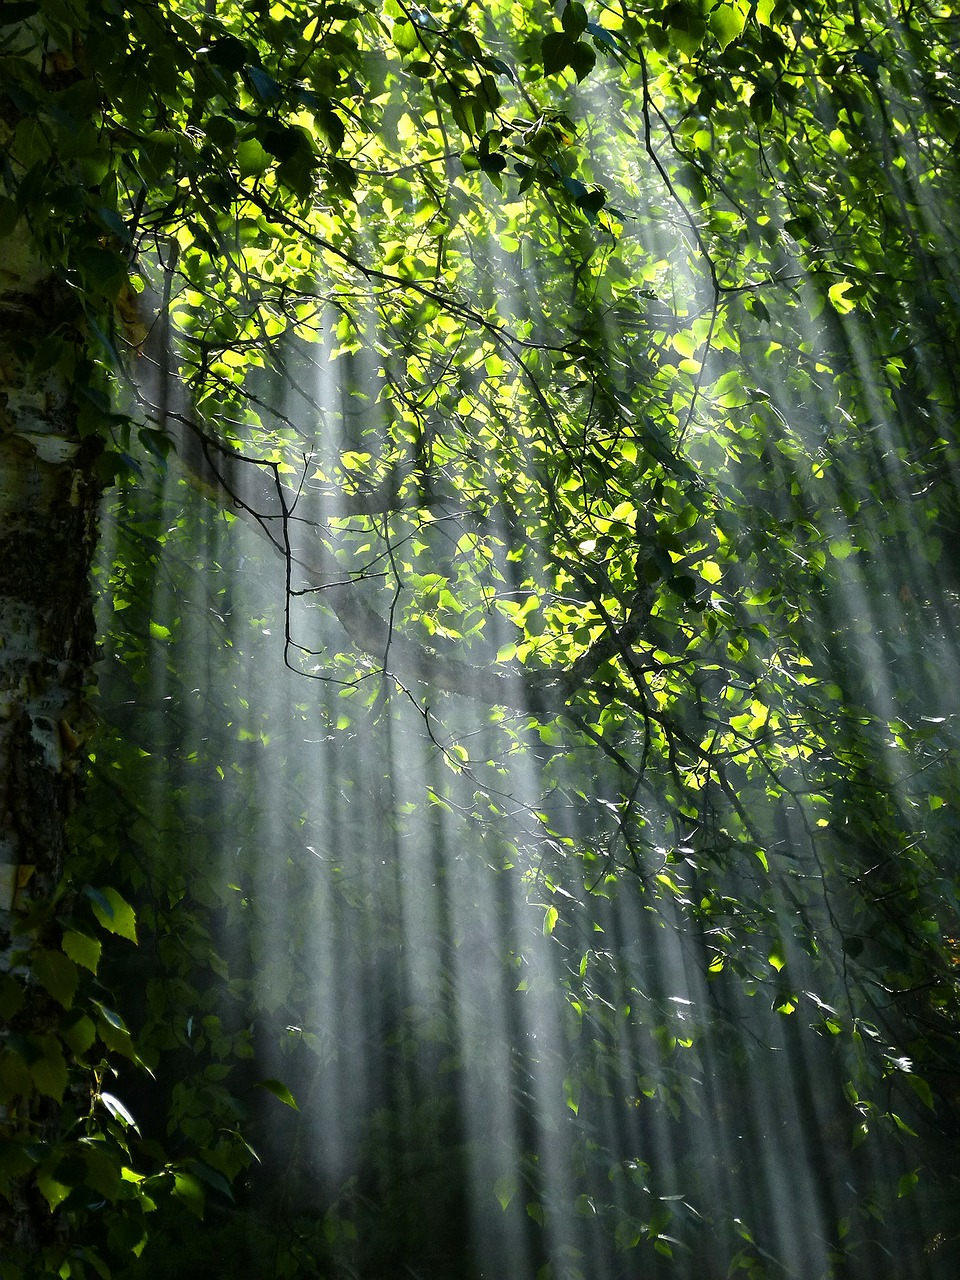
\includegraphics[width=\paperwidth,height=\paperheight]{bg_title_page}};
    \vspace{0.666\textheight} % height of the devil
    
    {\hspace{0pt}\vspace{0pt}\begin{tikzpicture}[scale=\paperwidth/1cm, overlay]
        \filldraw[draw=none,fill=white]
        (0, 0)
        -- (0.65838,0) 
        -- (0.71534285714,-0.1) 
        -- (0.7577,-0.0215)
        -- (0.8001, -0.1)
        -- (0.8571,0)
        -- (1, 0)
        -- (1, -0.45)
        -- (0, -0.45);

        \node[opacity=1,inner sep=0pt] at (0.7577, -0.15){
\includegraphics[width=6cm]{logotype}};
        \node[text width=15cm] at (0.39,-0.15) {\sffamily\fontsize{40}{10}\selectfont\textcolor{id7-aubergine}{Regular Expression\\\vspace{0.2cm}Refinement Types}};
        \end{tikzpicture}}
    
    {\par}
    \vspace{1.25cm}
    \vspace{3.5cm}
    {\hspace{0.75cm}\Huge \sffamily Progress Report}
    \vspace{0.16cm}
    {\par}
    {\hspace{0.75cm}\large \sffamily Adam Williams}
    
    \vspace{0cm}
    {\par}
    {\hspace{0.75cm}\large \sffamily Supervisor: Michael Gale}
    \vfill
\end{titlepage}
\restoregeometry
\restorepagecolor

\tableofcontents
\pagebreak[5]
    
    \section{Introduction}
    
    Within type systems, refinement types allow for predicate-based constraints to be applied to type definitions in order to restrict the domain of elements which belong to the type.
    
    For example, a local variable used to store natural numbers could be constrained via $\{n: \mathbb{N}\ | n \leq 5\}$. Only $\{0, 1, 2, 3, 4, 5\}$ would be permitted for values of $n$ under this refinement type.
    
    This project applies refinement types to strings which enforce membership of $L(R)$ for some regular expression $R$. For example, $\{s: \Sigma^* | s \in L(ab+)\}$ \footnote{For some regular expression $R$, $L(R)$ is used to denote the language that it accepts)} would allow \texttt{"ab"} to be assigned as a value of some variable $s$, but not \texttt{"a"}. This is motivated by the use of regular expressions as a validation mechanism to provide security in systems that handle user input. Designing a proof-of-concept language with syntax for expressing such refinement types and implementing a type checker will allow for the feasibility of such compile-time checks to be evaluated.

    Per the specification included in Appendix \ref{spec}, Weeks 1-9 of the project were scheduled to involve implementing and testing a prototype parser and type checker for the language.
    
    \section{Progress}
    
    Early on in the project lifetime it was decided to begin work on a phase 1 prototype with a simplified goal to gain some experience working with refinement types and type checkers in general. Once complete, work would continue in a 2nd phase which introduced regular expressions.
    
    The project is currently ahead of schedule. By week 7, both phases 1 and 2 have been completed to a satisfactory standard.
    
    \subsection*{Phase 1}
    
    Prototype work began with simple refinement types which could be applied to natural numbers. The final syntax was similar to the example presented in the specification:
    
    \begin{minted}{javascript}
function Main(id: uint): uint[< 4] {
    // A simple function declaration, returns an int less than 4
    return 0
}
function StackOne(): uint[> 5] {
    // This function must return an unsigned int greater than 5
    return LookupUserById(1)
}
    \end{minted}
    
    As the \texttt{Main()} function returns an integer less than 4, a violation is present within \texttt{StackOne()} where it is returned. This violation arises because \texttt{StackOne}'s return type is constrained to be greater than 5.
    
    Running this simple program with the prototype tool yields the following output:
    

    \termbox{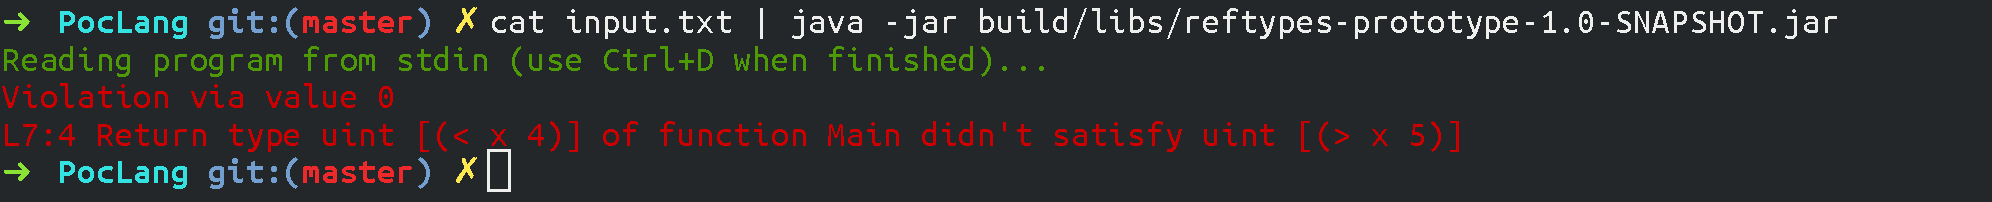
\includegraphics[width=\linewidth]{term1}}
    
    The prototype tool has found a valid value (here, $0$) which satisfies $x < 4$ but violates $x > 5$. If integrated into a ``real'' programming language, this would be identified at compile time and prevent successful compilation.
    
    This initial version of the prototype which operated exclusively on the natural numbers was built using the following tools, libraries and languages:
    
    \begin{description}
        \item[JavaSMT] Library which provides an abstraction layer over a variety of different SMT solvers (such as Z3 and MathSAT) and provides added type safety \citep{karpenkov2016javasmt}.
        \item[ANTLR 4] An $LL(*)$ lexer and parser generator which can target languages such as Java, Go and C\# \citep{parr2011ll}. In the initial prototype, ANTLR was used to generate a combined lexer-parser using a composite grammar in which both non-terminals and terminal symbols (tokens) are specified.
        \item[JUnit] A unit testing framework for Java. Used to build a collection of unit and integration tests to support refactoring and a test-driven development approach.
        \item[Gradle] Industry-standard build automation system which co-ordinates the grammar generation, Java class compilation, construction of a JAR file with shaded dependencies and running the unit tests.
        \item[IntelliJ IDEA] An advanced Java IDE with leading code inspection and analysis capabilities \citep{ideainspections} \citep{Jemerov:2008:IRI:1636642.1636655}. Used in conjunction with the official ANTLR plugin which provides grammar syntax highlighting and analysis.
    \end{description}

    The general steps involved in the process are described below.
    
    \tikzstyle{line} = [draw, -latex']
    \tikzset{arrow/.style={
            minimum height=1.2cm,%
            inner sep=1em,
            shape=signal,
            signal from=west,
            signal to=east,
            signal pointer angle=110,
            text depth=.25ex,
            text height=1.5ex,
            fill=skyblue,
            baseline,
            text centered, text=white
    }}
    \tikzset{arrowcur/.style={
            fill=id7-sky-blue-accent
    }}
    \begin{figure}[H]

            \begin{tikzpicture}[node distance=-\pgflinewidth, auto]
            \sffamily{
                \begin{scope}[start chain=transition going right,node distance=-\pgflinewidth]
                \node [arrow, arrowcur, on chain] {\faCogs{} \textbf{Parsing}};
                \node [arrow, on chain] {\faSearch{} Initial walk};
                \node [arrow, on chain] {\faSearch{} Final walk};
                \node [arrow, on chain] {\faCheckCircle{} Type checking};
                \node [arrow, on chain] {\faFileText{} Report};
                \end{scope}
            }
            \end{tikzpicture}

    \end{figure}
    

    In the \textbf{Parsing} step, the ANTLR parser is used to generate a parse tree from the input program. For example, consider the following simple function declaration:
    
    \begin{minted}{javascript}
function LookupUserById(id: uint[> 1]): uint {
    return 1*1
}
    \end{minted}
    
    % Insert tikz tree   
    
    For the phase 1 prototype, the lexer and parser are both generated from the same grammar file.
\bibliographystyle{agsm}
\bibliography{references}

\begin{appendices}
\titleformat{\section}
{\normalfont\sffamily\huge\color{id7-aubergine}}
{Appendix \thesection{} -- }{0em}{}
\section{Specification}

The original specification as submitted at the start of Term 1 is included overleaf.
\label{spec}
\end{appendices}
\includepdf[pages=2-]{../specification/spec.pdf}


\end{document}
